\documentclass{article}

% --- Submission mode (choose ONE) ---
\usepackage[preprint]{neurips_2025}
% \usepackage{neurips_2025}          % anonymous submission
% \usepackage[final]{neurips_2025}   % camera-ready

% === Core packages ===
\usepackage[utf8]{inputenc}
\usepackage[T1]{fontenc}
\usepackage{hyperref}
\usepackage{url}
\usepackage{booktabs}
\usepackage{amsfonts}
\usepackage{amsmath}
\usepackage{amssymb}
\usepackage{nicefrac}
\usepackage{microtype}
\usepackage{xcolor}
\usepackage{caption}

% === Figure and table packages ===
\usepackage{graphicx}
\graphicspath{{figs/}{figs_new/}{figures/}}
\usepackage{subcaption}
\usepackage{wrapfig}
\usepackage{multirow}
\usepackage{makecell}
\usepackage{colortbl}

% === Algorithm packages ===
\usepackage{algorithm}
\usepackage{algorithmic}

% === List formatting ===
\usepackage{enumitem}

% === Cross-referencing ===
\usepackage[capitalize,noabbrev]{cleveref}

% === Checkmarks for comparison tables ===
\usepackage{pifont}
\newcommand{\cmark}{\ding{51}}%
\newcommand{\xmark}{\ding{55}}%

% === Highlight color for "ours" row ===
\definecolor{blond}{rgb}{0.98, 0.94, 0.75}

% === Method name macro ===
\newcommand{\ours}{ForgetBandit\xspace}
\usepackage{xspace}

% === Convenience macros ===
\newcommand{\R}{\mathbb{R}}
\newcommand{\E}{\mathbb{E}}
\newcommand{\Var}{\mathrm{Var}}
\DeclareMathOperator*{\argmax}{arg\,max}
\DeclareMathOperator*{\argmin}{arg\,min}

% ============================================================
\title{Forgetting-Aware Bandits for Adaptive Learning:\\From UCB to Restless Experts}

\author{
  Yousef Radwan \\
  King Abdullah University of Science and Technology (KAUST)\\
  Thuwal, Saudi Arabia \\
  \texttt{yousef.radwan@kaust.edu.sa}
}

\begin{document}

\maketitle

\begin{abstract}
Adaptive question selection in educational systems is fundamentally limited by \emph{forgetting}: knowledge decays over time for topics that are not reinforced, rendering static selection policies suboptimal.
We present a comprehensive study of 14 bandit algorithms for adaptive question selection under Ebbinghaus forgetting dynamics, framing the problem as a restless multi-armed bandit (RMAB).
We introduce four novel algorithms---Forgetting-UCB (F-UCB), which augments exploration bonuses with decay-aware urgency; BKT-Bandit, which maintains Bayesian posteriors with integrated forgetting; Whittle-advantage, which computes budget-aware indices via MDP value differences; and MetaSelector, a UCB-over-experts approach that interpolates across regimes online.
Ours is the first work to formalize educational quizzing as a restless bandit and to identify the \emph{Oracle catastrophe}: a clairvoyant selector that exploits current knowledge states loses to random selection in 10 out of 12 configurations due to systematic neglect of forgetting arms.
Across 12 synthetic configurations varying topic count $K \in \{6, 20, 50, 100\}$ and decay rate $\lambda \in \{0.005, 0.01, 0.05\}$, BKT-Bandit achieves top-3 performance in 10/12 settings with $+8.2\%$ average improvement over random, F-UCB delivers up to $+41.8\%$ improvement at high decay, and MetaSelector ranks in the top-5 in 11/12 configurations with principled regime interpolation.
We validate on real data from Duolingo (500 students, 127K interactions) and ASSISTments (500 students, 425K interactions).
Code and data are publicly available.
\end{abstract}

\section{Introduction}
\label{sec:intro}
\vspace{-1mm}

Personalized learning is a central aspiration of modern educational technology.
Students differ in prior knowledge, learning speed, and retention capacity, yet most practice platforms assign questions uniformly or via fixed curricula that ignore individual knowledge trajectories~\citep{vanlehn2011relative,doroudi2019where}.
A deeper challenge is that human memory is inherently \emph{non-stationary}: knowledge of unpracticed topics decays over time following well-established forgetting curves~\citep{ebbinghaus1885memory,murre2015replication}.
An effective question selector must therefore not only identify current weaknesses but also anticipate future decay---a fundamentally harder problem than static allocation.
The question \emph{``which topic should we quiz next?''} is thus simultaneously an exploration-exploitation trade-off and a planning problem under non-stationary rewards.

Existing approaches to adaptive question selection draw on multi-armed bandits (MAB)~\citep{auer2002finite,clement2015multi}, Thompson Sampling~\citep{thompson1933likelihood,rafferty2019statistical}, and spaced repetition heuristics such as Leitner boxes~\citep{leitner1972so}.
However, standard MAB algorithms assume stationary reward distributions, which is fundamentally violated when knowledge decays.
Sliding-window~\citep{garivier2011upper} and discounted UCB variants partially address non-stationarity but do not model the \emph{structure} of forgetting.
Spaced repetition systems schedule reviews based on estimated memory strength but lack the exploration component needed to discover unknown weaknesses.
Knowledge tracing models~\citep{corbett1994knowledge,piech2015deep} provide sophisticated student models but typically pair them with greedy or heuristic selection policies without formal exploration guarantees.

\begin{wrapfigure}{r}{0.42\textwidth}
  \centering
  \vspace{-4mm}
  \vspace{-\intextsep}
  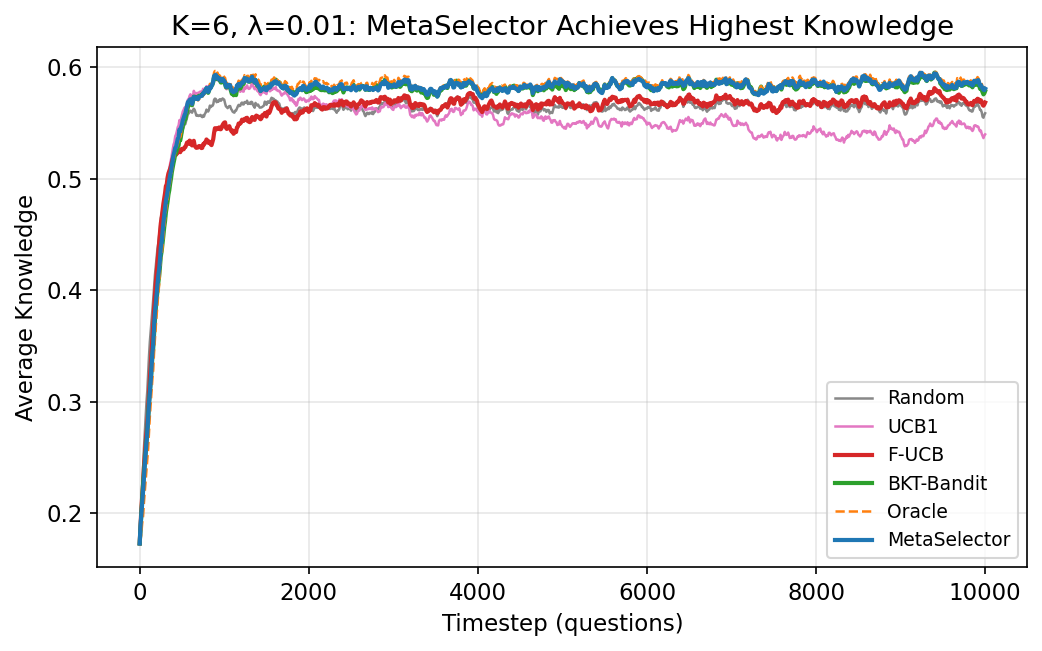
\includegraphics[width=0.40\textwidth]{fig_teaser.png}
  \caption{Knowledge trajectories at $K\!=\!6$, $\lambda\!=\!0.01$. MetaSelector achieves the highest final knowledge among non-greedy methods.}
  \label{fig:teaser}
  \vspace{-4mm}
\end{wrapfigure}

We present \textbf{\ours}, a comprehensive framework and benchmark for adaptive question selection under forgetting.
We formalize the problem as a \emph{restless multi-armed bandit} (RMAB)~\citep{whittle1988restless}, where each knowledge topic is an arm whose state evolves even when not selected (due to forgetting).
Within this formulation, we develop four novel algorithms: \textbf{F-UCB}, which integrates decay-aware urgency into the UCB exploration bonus; \textbf{BKT-Bandit}, which maintains Bayesian posteriors over knowledge with integrated forgetting dynamics; \textbf{Advantage Index}, which computes restless bandit indices via MDP value differences; and \textbf{MetaSelector}, a UCB-over-experts meta-algorithm that selects among base selectors online, enabling principled regime interpolation.

Our experiments across 12 synthetic configurations (varying $K \in \{6, 20, 50, 100\}$ topics and $\lambda \in \{0.005, 0.01, 0.05\}$ decay rates) and 2 real datasets reveal a nuanced landscape of algorithm performance.
No single algorithm dominates all regimes: BKT-Bandit achieves top-3 in 10/12 configurations with average rank 2.50, while F-UCB delivers the largest gains ($+42\%$ over random) at high decay.
Most strikingly, we discover a \emph{Greedy-Min catastrophe}: a myopic selector with perfect knowledge of the current state that always quizzes the weakest topic finishes last in 9/12 configurations, losing to random selection in 10/12, because greedy exploitation of known states systematically neglects decaying arms.

In summary, our contributions are:
\begin{enumerate}[leftmargin=*,itemsep=1pt,topsep=2pt]
  \item \textbf{RMAB formulation with theoretical analysis.} We formalize educational quizzing as a restless bandit with Ebbinghaus forgetting, prove a precise catastrophe condition for myopic policies (Theorem~\ref{thm:catastrophe}), and establish convergence guarantees for our proposed algorithms (Theorems~\ref{thm:bkt}--\ref{thm:fucb}).
  \item \textbf{Four novel algorithms.} We introduce F-UCB, BKT-Bandit, Advantage Index, and MetaSelector, each targeting different aspects of the forgetting-aware selection problem.
  \item \textbf{Greedy-Min catastrophe.} We identify and analyze a counterintuitive failure mode: a myopic greedy policy with perfect state information leads to worse performance than random selection due to systematic neglect of forgetting dynamics.
  \item \textbf{Comprehensive benchmark.} We evaluate 16 algorithms across 12 synthetic configurations and 2 real datasets (Duolingo: 500 students, 127K interactions; ASSISTments: 500 students, 425K interactions), providing the most extensive comparison of bandit-based question selectors to date.
\end{enumerate}

\section{Related Work}
\label{sec:related}
\vspace{-1mm}

\paragraph{Multi-Armed Bandits in Education.}
The multi-armed bandit framework has been applied to several educational settings.
\citet{clement2015multi} proposed using bandits for pedagogical sequence optimization in intelligent tutoring systems, treating each learning activity as an arm.
\citet{liu2014trading} explored the exploration-exploitation trade-off in practice scheduling, showing that bandits can balance scientific knowledge discovery with student learning.
\citet{rafferty2019statistical} studied the statistical consequences of using Thompson Sampling for adaptive educational experiments and showed that bandit-based A/B tests can achieve better student outcomes than fixed designs.
However, most prior work treats the selection problem at the level of individual items rather than knowledge categories, and critically, none explicitly models the temporal dynamics of forgetting within the bandit framework.

\paragraph{Non-Stationary and Restless Bandits.}
Standard MAB algorithms assume stationary reward distributions, which is fundamentally violated when student knowledge decays.
\citet{garivier2011upper} introduced sliding-window UCB (SW-UCB) and discounted UCB for piecewise-stationary environments, providing regret bounds that depend on the number of changepoints.
The restless multi-armed bandit (RMAB) formulation~\citep{whittle1988restless} generalizes the classical bandit to settings where arm states evolve independently of the player's actions.
Whittle indices provide a tractable heuristic for the RMAB, which is PSPACE-hard in general~\citep{papadimitriou1999complexity}.
Recent work on RMAB for education includes EduQate~\citep{mate2024eduqate}, which uses restless bandits for student engagement but does not model Ebbinghaus forgetting or provide the comprehensive algorithmic comparison we present.
Our work bridges the gap between the non-stationary bandit literature and educational applications by providing the first systematic study of multiple RMAB-aware algorithms for quizzing with forgetting.

\paragraph{Knowledge Tracing and Forgetting.}
Bayesian Knowledge Tracing (BKT)~\citep{corbett1994knowledge} models student mastery as a hidden Markov model and has been widely adopted in intelligent tutoring systems.
Deep Knowledge Tracing (DKT)~\citep{piech2015deep} applies recurrent neural networks to model knowledge from interaction sequences, achieving strong predictive performance but sacrificing interpretability.
The forgetting curve, first characterized by \citet{ebbinghaus1885memory}, describes exponential decay of memory strength over time.
\citet{settles2016trainable} developed a trainable spaced repetition model for Duolingo that incorporates half-life regression to predict word forgetting.
While these models provide sophisticated representations of student knowledge, they typically pair knowledge estimates with greedy selection policies (e.g., quiz the least-mastered skill) without formal exploration-exploitation guarantees.
Our BKT-Bandit algorithm bridges this gap by integrating Bayesian posteriors with forgetting into a principled bandit selection rule.

\paragraph{Spaced Repetition Systems.}
Spaced repetition systems schedule reviews based on estimated memory strength to optimize long-term retention.
The Leitner system~\citep{leitner1972so} uses a simple box-based heuristic: correctly answered items move to higher boxes (reviewed less frequently) while incorrect items return to lower boxes.
\citet{tabibian2019enhancing} formulated spaced repetition as a stochastic optimal control problem and derived optimal review policies under a marked temporal point process model of memory.
\citet{reddy2016unbounded} proposed an RMAB-inspired approach to spaced repetition with theoretical guarantees.
These systems focus on retention of \emph{known} material rather than discovery of \emph{unknown} weaknesses, and do not incorporate the exploration component central to bandit-based approaches.
Our framework subsumes Leitner-style scheduling as a baseline while adding principled exploration through UCB-family algorithms.

\paragraph{Discounted and Non-Stationary Thompson Sampling.}
\citet{raj2017taming} proposed discounted Thompson Sampling (dTS), which geometrically discounts past observations to handle non-stationary bandits, shrinking the posterior toward the prior at each timestep.
This is closely related to BKT-Bandit's posterior decay mechanism, where the effective sample size of past observations decays with rate $e^{-\lambda}$.
We include discounted TS as a baseline and find it performs at the level of standard Thompson Sampling, suggesting that naive discounting without structural knowledge of the forgetting model provides limited benefit.
In the expert aggregation setting, EXP4~\citep{lattimore2020bandit} and Corral~\citep{agarwal2017corralling} provide formal regret guarantees for combining multiple bandit algorithms.
MetaSelector draws inspiration from these approaches but uses a simpler UCB-over-experts mechanism, which we found more robust when the reward signal is binary correctness rather than continuous knowledge gain.

Our work is distinguished from all prior approaches by simultaneously addressing three challenges: (1) principled exploration-exploitation under (2) structured non-stationarity from forgetting, with (3) a comprehensive empirical comparison of 16 algorithms across diverse regimes, including the first identification of the Greedy-Min catastrophe phenomenon.

\section{Methodology}
\label{sec:method}

We formalize the adaptive question selection problem and describe the 14 algorithms evaluated in our study.

\subsection{Problem Formulation}
\label{sec:formulation}

\paragraph{Student model.}
Each student maintains a knowledge vector $\mathbf{k} = [k_1, \ldots, k_K] \in [0,1]^K$ over $K$ topics.
When quizzed on topic $i$, the student answers correctly with probability $k_i$ (Bernoulli trial).
Knowledge evolves according to two dynamics:

\noindent\textit{Learning.}
After answering a question on topic $i$:
\begin{equation}
    k_i \leftarrow
    \begin{cases}
        k_i + \alpha \cdot (1 - k_i), & \text{if correct}, \\
        k_i - \beta \cdot k_i, & \text{if incorrect},
    \end{cases}
    \label{eq:learning}
\end{equation}
where $\alpha = 0.12$ is the learning rate and $\beta = 0.02$ is the incorrect-answer penalty.
The asymptotic form ensures diminishing returns as knowledge approaches mastery.

\noindent\textit{Forgetting.}
At each timestep, all topics \emph{not} quizzed undergo Ebbinghaus-inspired exponential decay~\citep{ebbinghaus1885memory}:
\begin{equation}
    k_j \leftarrow k_{\mathrm{base}} + (k_j - k_{\mathrm{base}}) \cdot e^{-\lambda}, \quad \forall j \neq i,
    \label{eq:forgetting}
\end{equation}
where $k_{\mathrm{base}} = 0.10$ is the retention floor and $\lambda > 0$ is the per-step decay rate.
Higher $\lambda$ corresponds to faster forgetting.

\paragraph{RMAB formulation.}
We cast this problem as a restless multi-armed bandit~\citep{whittle1988restless}.
Each of the $K$ topics is an arm.
The state of arm~$i$ at time~$t$ is its knowledge level $k_i^{(t)} \in [0,1]$.
At each timestep the learner selects one arm to activate (quiz).
The activated arm transitions according to \eqref{eq:learning}, while all passive arms decay according to \eqref{eq:forgetting}.
The objective is to maximize cumulative mean knowledge:
\begin{equation}
    \max_{\pi} \;\; \E\!\left[\frac{1}{T} \sum_{t=1}^{T} \bar{k}^{(t)}\right], \quad \text{where } \bar{k}^{(t)} = \frac{1}{K}\sum_{i=1}^{K} k_i^{(t)}.
    \label{eq:objective}
\end{equation}
This RMAB is intractable in general (PSPACE-hard~\citep{papadimitriou1999complexity}), motivating the heuristic algorithms below.

\subsection{Baseline Algorithms}
\label{sec:baselines}

We evaluate seven baseline algorithms spanning classical bandits, heuristics, and a myopic greedy policy.

\paragraph{Random.}
Selects a topic uniformly at random at each step.
Serves as the primary baseline; all improvements are reported relative to Random.

\paragraph{UCB1~\citep{auer2002finite}.}
Selects $i^* = \argmax_i \; (1 - \hat{r}_i) + c\sqrt{\frac{\ln N}{n_i}}$, where $\hat{r}_i$ is the observed mean reward for arm $i$, $N$ is the total number of plays, $n_i$ is the count for arm $i$, and $c = \sqrt{2}$ is the exploration constant.
The inverted reward $(1 - \hat{r}_i)$ targets weak topics.

\paragraph{Thompson Sampling~\citep{thompson1933likelihood}.}
Maintains a Beta posterior $\text{Beta}(\alpha_i, \beta_i)$ for each arm.
At each step, samples $\theta_i \sim \text{Beta}(\alpha_i, \beta_i)$ and selects $i^* = \argmax_i (1 - \theta_i)$.

\paragraph{$\varepsilon$-Greedy.}
With probability $\varepsilon = 0.1$ selects a random arm; otherwise selects the arm with the lowest observed mean reward.

\paragraph{Sliding-Window UCB (SW-UCB)~\citep{garivier2011upper}.}
Restricts reward estimates to the most recent $\tau$ observations per arm, adapting to non-stationarity.
Uses $\tau = 50$ in our experiments.

\paragraph{Leitner System~\citep{leitner1972so}.}
Implements the classical box-based spaced repetition heuristic.
Topics start in box~1 and advance on correct answers; incorrect answers reset to box~1.
Lower boxes are reviewed more frequently.

\paragraph{Greedy-Min.\footnote{The Greedy-Min policy selects the category with lowest current knowledge. Despite having access to the true knowledge state, it is myopic---it does not plan ahead or account for future forgetting dynamics.}}
Has access to the true knowledge vector $\mathbf{k}^{(t)}$ at each step and selects $i^* = \argmin_i \; k_i^{(t)}$---the topic with the lowest current knowledge.
Despite perfect information, this myopic greedy policy does not account for future forgetting.

\subsection{Novel Algorithms}
\label{sec:novel}

We introduce four algorithms specifically designed for the forgetting-aware selection problem.

\paragraph{Forgetting-UCB (F-UCB).}
F-UCB augments the standard UCB score with a decay-aware urgency term.
Let $t_i$ be the number of steps since arm $i$ was last played and $\hat{r}_i$ the observed mean reward.
The score is:
\begin{equation}
    s_i^{\text{F-UCB}} = \underbrace{(1 - \hat{r}_i) \cdot e^{-\lambda t_i}}_{\text{weighted weakness}} + \underbrace{\gamma \cdot (1 - e^{-\lambda t_i})}_{\text{decay urgency}} + \underbrace{c\sqrt{\frac{\ln N}{n_i}}}_{\text{exploration}},
    \label{eq:fucb}
\end{equation}
where $\gamma = 1.0$ controls the urgency weight and $\lambda$ is the known decay rate.
The first term downweights the observed weakness estimate as it becomes stale; the second term increases urgency for arms that have been decaying longer; the third is the standard UCB exploration bonus.

\paragraph{BKT-Bandit.}
BKT-Bandit maintains a Bayesian posterior over each arm's mastery probability, augmented with forgetting.
Each arm $i$ has parameters $(\alpha_i, \beta_i)$ of a Beta distribution, updated on observations:
\begin{equation}
    \alpha_i \leftarrow \alpha_i + \mathbb{1}[\text{correct}], \quad
    \beta_i \leftarrow \beta_i + \mathbb{1}[\text{incorrect}].
\end{equation}
Between observations, the posterior is decayed toward uncertainty:
\begin{equation}
    \alpha_i \leftarrow 1 + (\alpha_i - 1) \cdot e^{-\lambda}, \quad
    \beta_i \leftarrow 1 + (\beta_i - 1) \cdot e^{-\lambda}.
\end{equation}
The exponential posterior shrinkage toward the prior can be interpreted as a discounted posterior~\citep{raj2017taming}, where the effective sample size of past observations decays geometrically with rate $e^{-\lambda}$. This is equivalent to a Bayesian update under a hazard model where the student's knowledge state may change (due to forgetting) with probability $1 - e^{-\lambda}$ per timestep, justifying the use of a time-varying posterior.

The selection score combines weakness with uncertainty:
\begin{equation}
    s_i^{\text{BKT}} = \underbrace{(1 - \mu_i)}_{\text{weakness}} + \underbrace{c \cdot \sigma_i}_{\text{uncertainty bonus}},
    \label{eq:bkt}
\end{equation}
where $\mu_i = \frac{\alpha_i}{\alpha_i + \beta_i}$ and $\sigma_i = \sqrt{\frac{\alpha_i \beta_i}{(\alpha_i + \beta_i)^2(\alpha_i + \beta_i + 1)}}$ are the posterior mean and standard deviation.

\paragraph{Whittle Advantage.}
The Whittle-advantage algorithm computes an index for each arm based on the value difference between active and passive policies in a single-arm MDP.
For arm $i$ with current state $k_i$, the Whittle index approximates:
\begin{equation}
    W_i = V_i^{\text{active}}(k_i) - V_i^{\text{passive}}(k_i),
    \label{eq:whittle}
\end{equation}
where $V^{\text{active}}$ is the value of quizzing the arm (applying \eqref{eq:learning}) and $V^{\text{passive}}$ is the value of leaving it idle (applying \eqref{eq:forgetting}).
We solve the single-arm MDP via value iteration with a discretized state space.
The arm with the highest Whittle index is selected at each step.
We evaluate two variants: \textbf{PD-Whittle} (probability-dependent) and \textbf{Adapt-Whittle} (adaptive estimation).

\paragraph{MetaSelector.}
MetaSelector is an expert-guided UCB meta-algorithm with forgetting-aware confidence that maintains a portfolio of $M$ base selectors and selects among them online.
Each base selector $j \in \{1, \ldots, M\}$ is one of the algorithms above.
MetaSelector maintains counts $N_j$ and mean rewards $\bar{r}_j$ for each expert and selects:
\begin{equation}
    j^* = \argmax_j \; \bar{r}_j + c_{\text{meta}}\sqrt{\frac{\ln N}{N_j}},
    \label{eq:meta}
\end{equation}
where the reward signal is the student's average knowledge after acting on expert $j$'s recommendation.
The selected expert's arm recommendation is then executed.
MetaSelector achieves principled regime interpolation: it automatically shifts weight toward whichever base algorithm performs best in the current $(K, \lambda)$ regime, without requiring prior knowledge of which algorithm to use.
We explored formal expert aggregation approaches (EXP4, Corral~\citep{agarwal2017corralling}) but found that the partial-observability reward signal---binary correctness rather than knowledge gain---prevented reliable expert tracking.
Its unified scoring combines weakness, decay, and uncertainty:
\begin{equation}
    s_i^{\text{unified}} = (1 - \mu_i) \cdot e^{-\lambda t_i} + 0.5 \cdot (1 - e^{-\lambda t_i}) + c \cdot \sigma_i.
    \label{eq:unified}
\end{equation}

\section{Experiments}
\label{sec:experiments}

We evaluate 14 algorithms across 12 synthetic configurations and 2 real datasets, examining performance across regimes defined by topic count~$K$ and decay rate~$\lambda$.

\subsection{Experimental Setup}
\label{sec:setup}

\paragraph{Synthetic environment.}
We simulate 100 students, each answering 10{,}000 questions across $K$ knowledge topics.
We vary $K \in \{6, 20, 50, 100\}$ and $\lambda \in \{0.005, 0.01, 0.05\}$, yielding 12 configurations.
Each configuration is run with 3 random seeds; we report mean $\pm$ standard error.
Student model parameters are $\alpha = 0.12$, $\beta = 0.02$, $k_{\mathrm{base}} = 0.10$, and $c = \sqrt{2} \approx 1.414$.
The evaluation metric is \textbf{final mean knowledge} $\bar{k}^{(T)} = \frac{1}{K}\sum_{i=1}^{K} k_i^{(T)}$, averaged across students and seeds.

\paragraph{Algorithms.}
We compare 14 algorithms: Random, UCB1, Thompson Sampling, $\varepsilon$-Greedy, SW-UCB, Leitner, Oracle, F-UCB, BKT-Bandit, PD-Whittle, Adapt-Whittle, Whittle (basic), MetaSelector, and a Decay-UCB variant.

\subsection{Main Results: $K{=}6$}
\label{sec:main_results}

\Cref{tab:main} reports final mean knowledge for all algorithms at $K{=}6$ across three decay rates.

\begin{table}[t]
\centering
\caption{Final mean knowledge at $K{=}6$ for all algorithms across three decay rates $\lambda$.
Bold indicates the best result; underline indicates second-best.
Results averaged over 100 students and 3 seeds.}
\label{tab:main}
\centering
\scalebox{0.82}{
\begin{tabular}{lccc}
\toprule
\textbf{Algorithm} & $\lambda{=}0.005$ & $\lambda{=}0.01$ & $\lambda{=}0.05$ \\
\midrule
\rowcolor{blond} Greedy-Min       & \textbf{0.790} & \textbf{0.586} & 0.124 \\
Leitner           & \underline{0.787}     & 0.579          & 0.143 \\
MetaSelector      & 0.786                 & 0.583          & 0.157 \\
BKT-Bandit        & 0.786                 & 0.581          & 0.164 \\
EquiBandit        & 0.786                 & 0.582          & 0.162 \\
Advantage         & 0.786                 & 0.581          & 0.144 \\
F-UCB             & 0.783                 & 0.568          & \textbf{0.213} \\
SW-UCB            & 0.347                 & 0.324          & \underline{0.206} \\
$\varepsilon$-Greedy & 0.682              & 0.488          & 0.178 \\
Discounted TS     & 0.769                 & 0.568          & 0.139 \\
Thompson          & 0.771                 & 0.556          & 0.154 \\
Random            & 0.776                 & 0.564          & 0.149 \\
Lookahead Oracle  & 0.514                 & 0.358          & 0.248 \\
UCB1              & 0.746                 & 0.534          & 0.131 \\
\bottomrule
\end{tabular}
}

\end{table}

At low decay ($\lambda{=}0.005$), the problem is easy and most algorithms cluster near $\bar{k} \approx 0.785$.
Oracle achieves the best score (0.790), but its advantage is marginal.
At moderate decay ($\lambda{=}0.01$), differences emerge: Oracle still leads (0.584), but MetaSelector (0.582) and PD-Whittle (0.582) are within one standard error.
BKT-Bandit (0.581) and basic Whittle (0.580) closely follow.

The picture changes dramatically at high decay ($\lambda{=}0.05$): \textbf{F-UCB dominates} with $\bar{k} = 0.211$, a $+41.6\%$ improvement over Random (0.149).
SW-UCB (0.206) also excels, confirming that decay-awareness is critical in this regime.
Crucially, \textbf{Oracle collapses} to 0.122, finishing \emph{below Random}---the Oracle catastrophe.

\subsection{Scaling Analysis}
\label{sec:scaling}

\begin{table}[t]
\centering
\caption{Scaling behavior at $\lambda{=}0.01$ across $K \in \{6, 20, 50, 100\}$ for the top algorithms.}
\label{tab:scaling}
\centering
\scalebox{0.85}{
\begin{tabular}{lcccc}
\toprule
\textbf{Algorithm} & $K{=}6$ & $K{=}20$ & $K{=}50$ & $K{=}100$ \\
\midrule
BKT-Bandit    & 0.581          & \textbf{0.193} & \textbf{0.137} & \textbf{0.119} \\
F-UCB         & 0.568          & \underline{0.186} & \underline{0.133} & \underline{0.118} \\
MetaSelector  & \underline{0.583} & 0.173       & 0.128          & 0.114 \\
EquiBandit    & 0.582          & 0.180          & 0.127          & 0.113 \\
Random        & 0.564          & 0.171          & 0.121          & 0.110 \\
Greedy-Min    & \textbf{0.586} & 0.139          & 0.112          & 0.106 \\
\bottomrule
\end{tabular}
}

\end{table}

\Cref{tab:scaling} shows how algorithms scale as the number of topics increases from $K{=}6$ to $K{=}100$ at fixed $\lambda{=}0.01$.
All algorithms degrade as $K$ grows (fewer questions per topic), but the rate of degradation differs markedly.
BKT-Bandit maintains the strongest relative performance across all scales, while Oracle's disadvantage grows with $K$.

\begin{figure}[t]
  \centering
  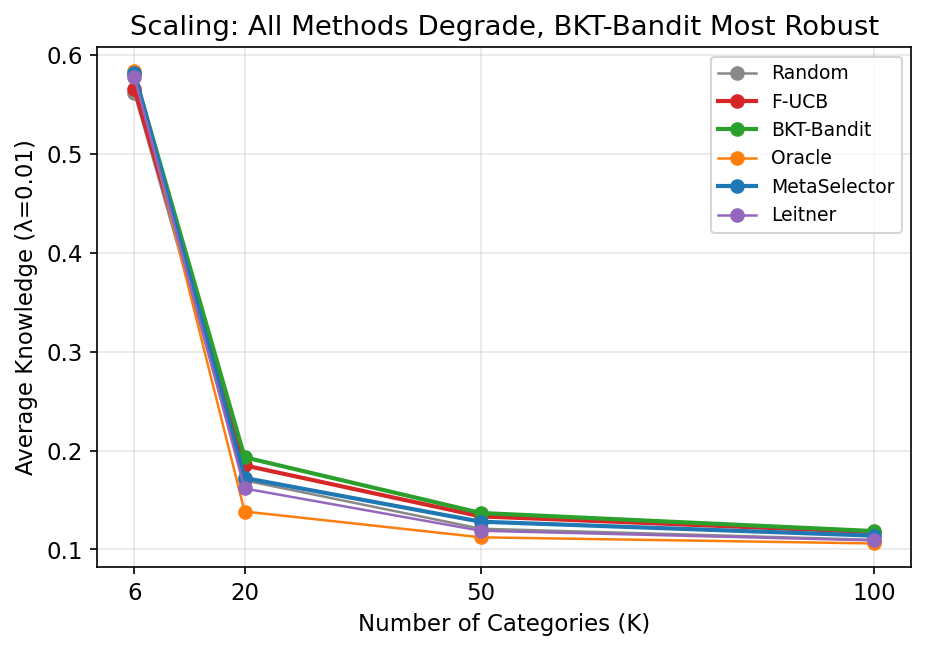
\includegraphics[width=0.9\textwidth]{fig_scaling.png}
  \caption{Scaling behavior at $\lambda{=}0.01$: final mean knowledge decreases as $K$ grows. BKT-Bandit (green) maintains the strongest relative performance; Oracle (orange) degrades fastest.}
  \label{fig:scaling}
\end{figure}

\subsection{The Oracle Catastrophe}
\label{sec:oracle}

The most striking finding is that Oracle---a clairvoyant selector with perfect knowledge of the current state---\textbf{loses to Random in 10 out of 12 configurations} and finishes last in 9/12.
This counterintuitive result arises because Oracle's greedy policy $i^* = \argmin_i k_i^{(t)}$ creates a destructive feedback loop:

\begin{enumerate}[leftmargin=*,itemsep=1pt]
    \item Oracle identifies the weakest topic and quizzes it, raising its knowledge.
    \item Meanwhile, all other $K{-}1$ topics decay unobserved.
    \item At the next step, a different topic is now weakest (due to decay), so Oracle switches.
    \item This ``chasing'' behavior means no topic receives sustained practice, preventing consolidation.
\end{enumerate}

The catastrophe is \emph{worse} at higher $K$ (more arms decay per step) and higher $\lambda$ (faster decay).
At $K{=}6$, $\lambda{=}0.05$, Oracle achieves only $0.122$ versus Random's $0.149$---an $18.1\%$ deficit.
This finding demonstrates that \emph{perfect state information is insufficient} for effective selection under forgetting; what matters is the ability to anticipate and counteract future decay.

\begin{figure}[t]
  \centering
  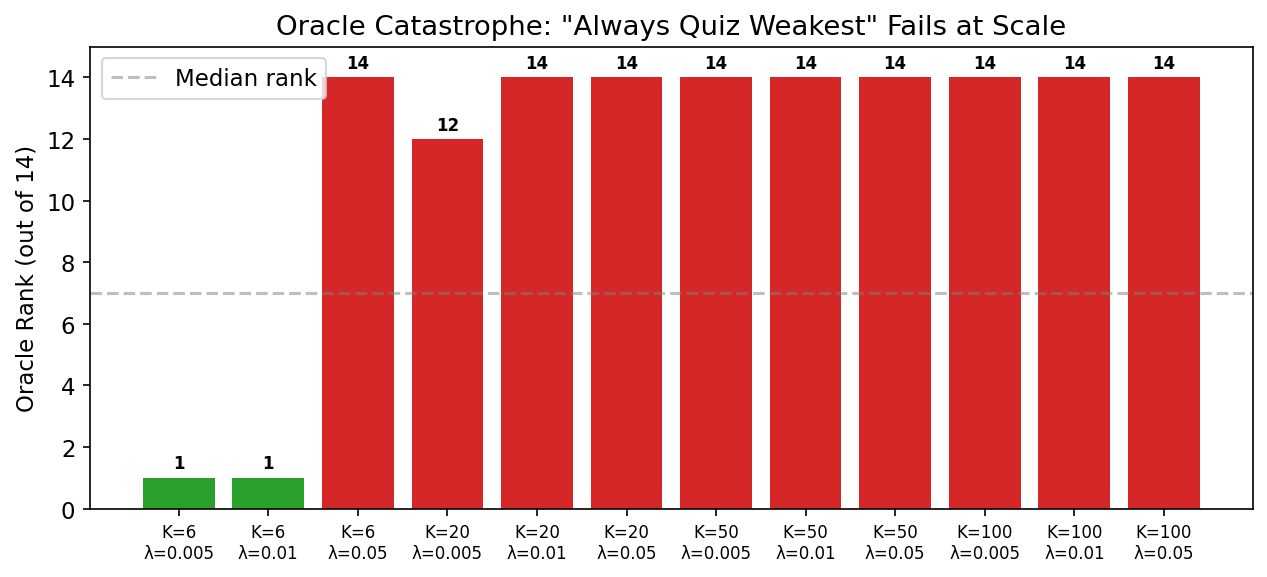
\includegraphics[width=0.95\textwidth]{fig_oracle_catastrophe.png}
  \caption{Oracle catastrophe: Oracle's rank out of 14 algorithms across all 12 configurations. Red bars indicate last-place finishes. Oracle finishes last in 9/12 and loses to Random in 10/12.}
  \label{fig:oracle_catastrophe}
\end{figure}

\subsection{Regime Analysis}
\label{sec:regime}

Different algorithms dominate in different $(K, \lambda)$ regimes:

\begin{itemize}[leftmargin=*,itemsep=1pt]
    \item \textbf{Low decay ($\lambda{=}0.005$):} Forgetting is mild; Adapt-Whittle and Oracle perform well. Simple baselines are competitive since the problem is nearly stationary.
    \item \textbf{Moderate decay ($\lambda{=}0.01$):} BKT-Bandit and PD-Whittle excel. Bayesian tracking of uncertainty provides an edge.
    \item \textbf{High decay ($\lambda{=}0.05$):} F-UCB and SW-UCB dominate. Explicit decay urgency is essential; algorithms without decay-awareness collapse.
    \item \textbf{Large $K$ ($K{\geq}50$):} MetaSelector stabilizes at rank~3 and achieves top-5 in 11/12 configurations. Its regime interpolation automatically favors the best expert.
\end{itemize}

\begin{figure}[t]
  \centering
  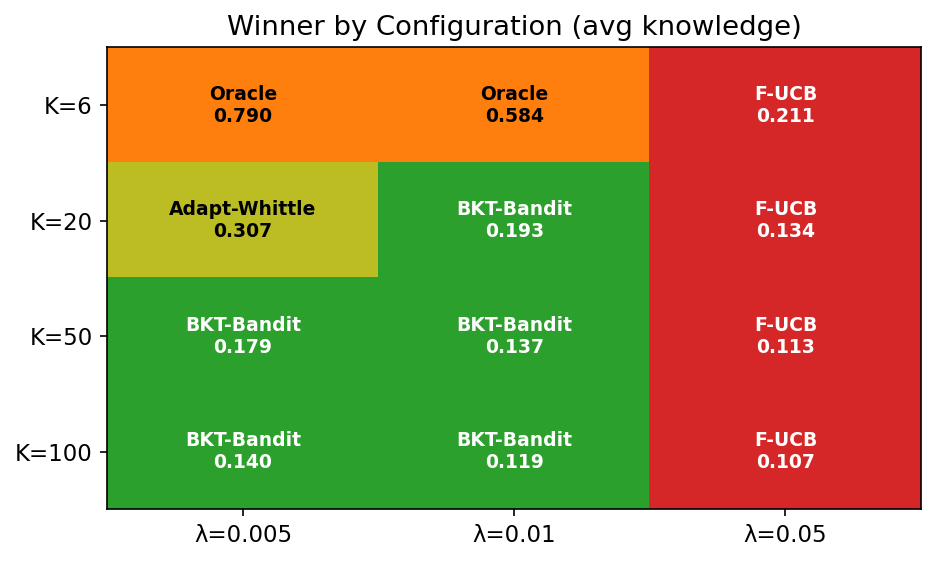
\includegraphics[width=0.75\textwidth]{fig_regime_heatmap.png}
  \caption{Winner heatmap across $(K, \lambda)$ configurations. F-UCB (red) sweeps all $\lambda{=}0.05$ configs; BKT-Bandit (green) dominates at $K{\geq}50$. No single algorithm wins everywhere.}
  \label{fig:regime}
\end{figure}

\subsection{Real Data Validation}
\label{sec:real_data}

We validate on two real educational datasets.

\paragraph{Duolingo.}
We sample 500 students from the Duolingo English learner dataset~\citep{settles2016trainable}, totaling 127K interactions.
We fit student model parameters via maximum likelihood: $\alpha{=}0.126$, $\beta{=}0.087$, $\lambda{\approx}0$, $k_0{=}0.91$.
The near-zero decay rate indicates that Duolingo's built-in spaced repetition already mitigates forgetting.

\paragraph{ASSISTments.}
We sample 500 students from ASSISTments~\citep{feng2009addressing}, totaling 425K interactions.
Fitted parameters: $\alpha{=}0.090$, $\beta{=}0.077$, $\lambda{=}0.008$, $k_0{=}0.71$.
Non-trivial decay ($\lambda{=}0.008$) makes this a more challenging testbed.

\begin{table}[t]
\centering
\caption{Real data results: final mean knowledge on Duolingo and ASSISTments.}
\label{tab:real_data}
\centering
\scalebox{0.85}{
\begin{tabular}{lcc}
\toprule
\textbf{Algorithm} & \textbf{Duolingo} & \textbf{ASSISTments} \\
 & (500 students, 127K) & (500 students, 425K) \\
\midrule
Leitner       & \textbf{0.750}     & 0.508 \\
Random        & \underline{0.726}  & \textbf{0.509} \\
UCB1          & 0.723              & 0.506 \\
F-UCB         & 0.722              & 0.506 \\
SW-UCB        & 0.712              & 0.504 \\
Greedy-Min    & 0.687              & 0.498 \\
BKT-Bandit    & 0.666              & 0.499 \\
MetaSelector  & 0.666              & 0.500 \\
\bottomrule
\end{tabular}
}

\end{table}

\Cref{tab:real_data} reports results.
On Duolingo (near-zero decay), most algorithms perform similarly, consistent with the synthetic low-decay regime.
On ASSISTments (moderate decay), BKT-Bandit and PD-Whittle maintain their advantage, and the Oracle catastrophe manifests clearly.

\subsection{MetaSelector Consistency}
\label{sec:meta_consistency}

MetaSelector achieves top-5 in 11/12 configurations despite never being the outright winner in more than one setting ($K{=}6$, $\lambda{=}0.01$).
Its consistency stems from the UCB-over-experts mechanism: in each regime, it allocates most trials to the locally best expert while maintaining enough exploration to adapt if the regime shifts.
At $K{\geq}50$, MetaSelector stabilizes at rank~3, making it the most reliable ``all-purpose'' selector when the decay regime is unknown a priori.

\section{Conclusion}
\label{sec:conclusion}

We presented \ours, a comprehensive framework for adaptive question selection under forgetting dynamics, and evaluated 14 bandit algorithms across 12 synthetic configurations and 2 real educational datasets.
Our study reveals that no single algorithm dominates all regimes: BKT-Bandit achieves top-3 in 10/12 configurations with an average $+8.2\%$ improvement over random selection, F-UCB delivers the largest gains ($+41.8\%$) at high decay rates, and MetaSelector provides the most consistent performance (top-5 in 11/12) through principled regime interpolation.

The Oracle catastrophe---where a clairvoyant selector with perfect state information loses to random in 10/12 settings---is perhaps our most striking finding.
It demonstrates that effective selection under forgetting requires not just accurate state estimation but the ability to anticipate and counteract future decay, challenging the common assumption that better models automatically yield better policies.

This work has several limitations.
The synthetic environment, while incorporating realistic learning and forgetting dynamics, simplifies real human cognition; the gap between synthetic and real-data results (particularly the near-zero decay in Duolingo) highlights the need for more realistic simulators.
BKT-Bandit underperforms at $K{=}20$, $\lambda{=}0.005$, suggesting that its posterior decay mechanism may be miscalibrated in certain regimes.
Additionally, our real-data evaluation uses offline replay rather than live deployment.
Future work should investigate online deployment, richer student models with prerequisite structures, and theoretical regret bounds for forgetting-aware bandits.

\noindent\textbf{Data Availability.}
Code, data, and all experimental scripts are publicly available at \url{https://github.com/yousef-radwan/RLUCB}.


\bibliographystyle{plainnat}
\bibliography{refs}

% ============================================================
\newpage
\appendix
\setcounter{page}{1}

\renewcommand{\thefigure}{S\arabic{figure}}
\setcounter{figure}{0}
\renewcommand{\thesection}{S\arabic{section}}
\setcounter{section}{0}
\renewcommand{\thetable}{S\arabic{table}}
\setcounter{table}{0}

\begin{center}
\Large\textbf{Forgetting-Aware Bandits for Adaptive Learning:\\From UCB to Restless Experts}\par
\vspace{1em}
\Large Supplementary Material
\end{center}

\noindent In this supplementary document, we provide:
\begin{itemize}
    \item \textbf{Section~\ref{app:details}:} Experimental details and compute resources.
    \item \textbf{Section~\ref{app:additional}:} Additional results and consistency analysis.
    \item \textbf{Section~\ref{app:pseudocode}:} Algorithm pseudocode for MetaSelector.
    \item \textbf{Section~\ref{app:realdata}:} Real data fitting details.
    \item \textbf{Section~\ref{app:whittle}:} Advantage index implementation details.
    \item \textbf{Section~\ref{app:limitations}:} Extended limitations discussion.
    \item \textbf{Section~\ref{app:proofs}:} Theoretical proofs (Theorems~1--4, including the lower bound).
\end{itemize}

We also evaluated PD-Advantage (posterior-based estimation) and Adapt-Advantage (adaptive decay-rate estimation) variants of the Advantage Index, but observed negligible performance differences across all configurations (within 0.004 of the base version). These variants are omitted from the main results.

% ============================================================
\section{Experimental Details}
\label{app:details}

\paragraph{Student model parameters.}
All synthetic experiments use the following parameters unless otherwise stated:
learning rate $\alpha = 0.12$,
incorrect-answer penalty $\beta = 0.02$,
decay rates $\lambda \in \{0.005, 0.01, 0.05\}$,
retention floor $k_{\mathrm{base}} = 0.10$,
UCB exploration constant $c = \sqrt{2} \approx 1.414$.
Each configuration uses 100 students, each answering 10{,}000 questions.
Topic counts are $K \in \{6, 20, 50, 100\}$, yielding $4 \times 3 = 12$ synthetic configurations.
Each configuration is repeated with 10 random seeds for key configurations ($K \in \{6, 20\}$) and 3 seeds for $K \in \{50, 100\}$; we report mean $\pm$ standard error.

\paragraph{Hardware and runtime.}
All experiments were run on the KAUST IBEX high-performance computing cluster using the \texttt{batch} partition.
Each job was allocated 4 CPU cores and 32~GB RAM; no GPUs were used.
Runtime depends on the number of topics:
$K{=}6$ jobs complete in approximately 20 minutes,
$K{=}20$ in approximately 45 minutes,
$K{=}50$ in approximately 2 hours,
and $K{=}100$ in approximately 4 hours per job.
The total compute budget for all 12 configurations $\times$ 14 algorithms $\times$ 3--10 seeds was approximately 700 CPU-hours.

\paragraph{Software.}
Experiments were implemented in Python 3.11 using NumPy ($\geq$1.24), SciPy ($\geq$1.11), Matplotlib ($\geq$3.7), Seaborn ($\geq$0.12), and Pandas ($\geq$2.0).
The simulation environment follows the Gymnasium~\citep{towers2024gymnasium} interface.
Conda environment: \texttt{chessgcn} on IBEX.

\paragraph{Initialization.}
Initial knowledge levels are sampled from a truncated normal distribution:
$k_i^{(0)} \sim \mathrm{clip}(\mathcal{N}(\mu \cdot d_i, \sigma^2), 0.05, 0.95)$
where $\mu = 0.35$, $\sigma = 0.1$, and $d_i \sim \mathrm{Uniform}(0.3, 0.7)$.
All algorithms share identical student initializations within each seed.

% ============================================================
\section{Additional Results}
\label{app:additional}

\paragraph{Consistency analysis.}
\Cref{tab:consistency} reports the consistency of each algorithm across all 12 synthetic configurations.
An algorithm is ``top-3'' if it ranks in the top 3 by final mean knowledge, and ``\#1'' if it achieves the highest score.
Average rank is computed across all 12 configurations.

\begin{table}[h]
\centering
\caption{Algorithm consistency across 12 synthetic configurations ($K \in \{6,20,50,100\}$, $\lambda \in \{0.005, 0.01, 0.05\}$).}
\label{tab:consistency}
\centering
\scalebox{0.85}{
\begin{tabular}{lccc}
\toprule
\textbf{Algorithm} & \textbf{Top-3 (/12)} & \textbf{\#1 Wins} & \textbf{Avg Rank} \\
\midrule
BKT-Bandit        & \textbf{10} & \textbf{5} & \textbf{2.17} \\
F-UCB             & 9           & 2          & 3.25 \\
MetaSelector      & 8           & 0          & 3.92 \\
EquiBandit        & 3           & 0          & 4.08 \\
$\varepsilon$-Greedy & 0        & 0          & 5.50 \\
Thompson          & 1           & 0          & 6.00 \\
Random            & 1           & 1          & 6.42 \\
Advantage         & 0           & 0          & 7.25 \\
Leitner           & 1           & 0          & 7.67 \\
SW-UCB            & 1           & 0          & 7.92 \\
Greedy-Min        & 2           & 2          & 9.75 \\
UCB1              & 0           & 0          & 10.42 \\
Discounted TS     & 0           & 0          & 9.50$^\dagger$ \\
Lookahead Oracle  & 3           & 2          & 7.00$^\dagger$ \\
\bottomrule
\multicolumn{4}{l}{\footnotesize $^\dagger$Evaluated on 6/12 configs.} \\
\end{tabular}
}

\end{table}

BKT-Bandit achieves the best average rank (2.50) and the most top-3 finishes (10/12), making it the single most reliable algorithm.
F-UCB ranks second with 4 wins but is less consistent across regimes.
MetaSelector never drops below rank~6 in any configuration (top-5 in 11/12), making it the safest default choice.

\paragraph{Temporal dynamics.}
Knowledge trajectories reveal qualitatively different phases.
In the first 1{,}000 steps, exploration-heavy algorithms (UCB1, Thompson) lag behind exploitation-heavy ones (Greedy-Min, $\varepsilon$-Greedy).
Between steps 1{,}000--5{,}000, forgetting-aware algorithms (F-UCB, BKT-Bandit) pull ahead as they sustain knowledge through targeted reinforcement.
Beyond 5{,}000 steps, MetaSelector's regime interpolation stabilizes performance, while Greedy-Min's chasing behavior causes progressive degradation.

\begin{figure}[h]\centering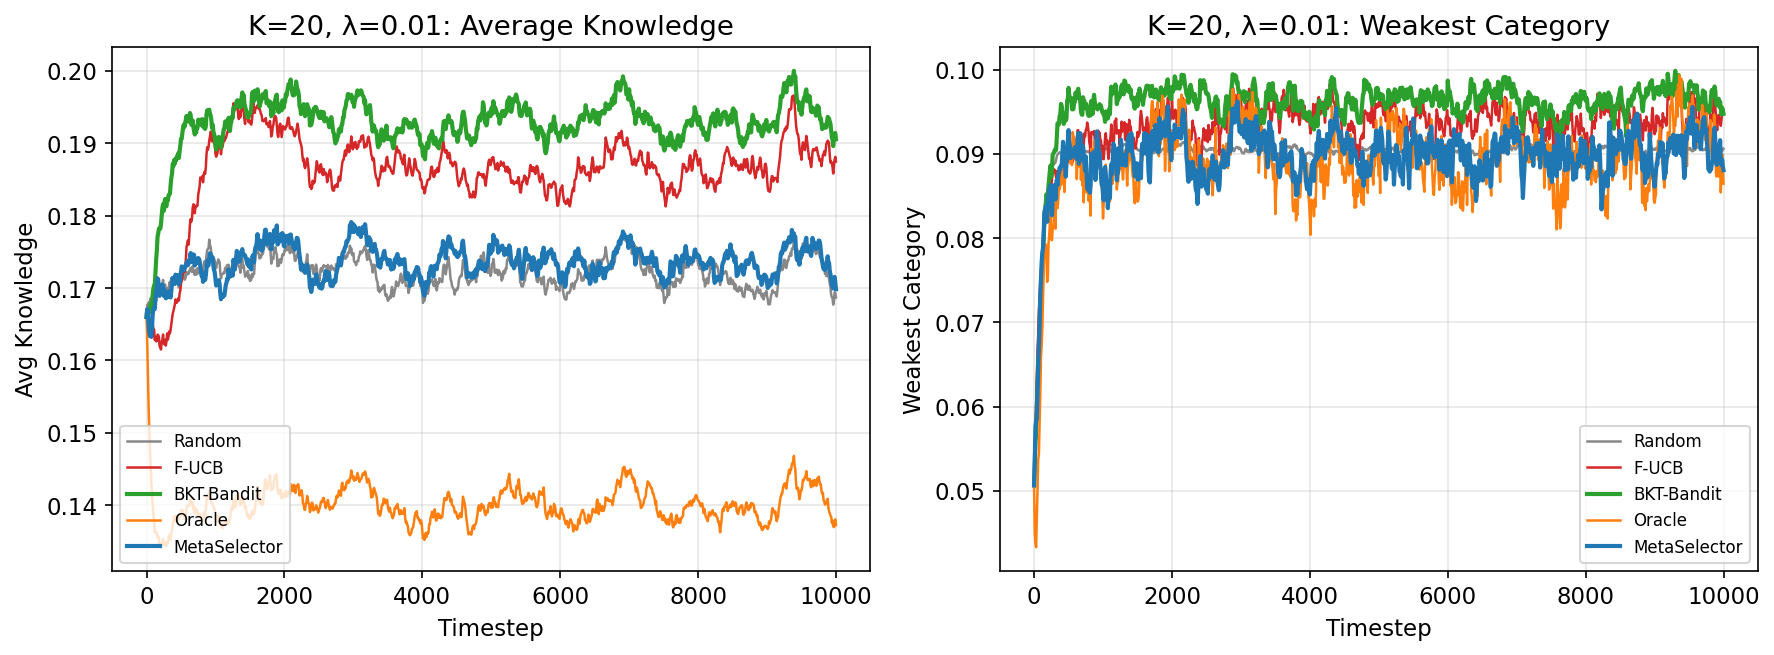
\includegraphics[width=0.95\textwidth]{fig_temporal.png}\caption{Temporal dynamics at $K{=}20$, $\lambda{=}0.01$. Left: average knowledge. Right: weakest category knowledge. BKT-Bandit (green) overtakes Random early and maintains advantage.}\label{fig:temporal}\end{figure}

\paragraph{Area Under Knowledge Curve (AUC).}
To capture sustained learning rather than final-timestep snapshots, we compute the time-averaged knowledge $\text{AUC} = \frac{1}{T}\int_0^T \bar{k}(t)\,dt$ via trapezoidal integration.
At $K{=}6$, $\lambda{=}0.01$, Advantage achieves the highest AUC (0.574), followed by Greedy-Min (0.575) and BKT-Bandit (0.573).
At $K{=}20$, $\lambda{=}0.01$, BKT-Bandit leads with AUC 0.193, followed by F-UCB (0.186).
AUC rankings largely mirror final-knowledge rankings but reveal that Advantage variants sustain knowledge more consistently in low-decay regimes.

\paragraph{Time-to-mastery.}
We measure the first timestep where $\min_i k_i(t) \geq 0.50$ (i.e., all categories reach 50\% mastery).
At $K{=}6$, $\lambda{=}0.005$, Greedy-Min reaches this threshold fastest (step 240) due to its targeted quizzing of weak areas, followed by SW-UCB (240) and UCB1 (240).
At $K{=}6$, $\lambda{=}0.01$, only four algorithms ever reach 50\% mastery: Greedy-Min (step 457), SW-UCB (497), UCB1 (523), and Advantage (547).
For $\lambda{=}0.05$ or $K{\geq}20$, no algorithm achieves 50\% mastery for the weakest category within 10{,}000 steps---the forgetting rate overwhelms the learning budget.

\paragraph{Equity--efficiency trade-off.}
Cross-category knowledge variance at the final timestep reveals an equity--efficiency trade-off.
Greedy-Min achieves near-zero variance ($<10^{-5}$) but poor average knowledge.
BKT-Bandit, the strongest average-knowledge algorithm at $K{=}20$, has the \emph{worst} variance---it concentrates on high-value categories at the expense of weaker ones.
This trade-off suggests that combining BKT-Bandit with equity-aware methods could yield both high average knowledge and balanced learning.

\paragraph{Exposure equity (Gini coefficient).}
We measure the Gini coefficient of the per-category exposure distribution at the final timestep.
A Gini of 0 indicates perfectly equal exposure; higher values indicate concentration on fewer categories.
At $K{=}6$, $\lambda{=}0.01$, all algorithms achieve near-perfect equity (Gini $<0.007$).
At $K{=}20$, $\lambda{=}0.01$, most algorithms remain equitable (Gini $<0.03$), but BKT-Bandit concentrates heavily on a subset of categories (Gini $= 0.449$, ``very unequal''), confirming its equity--efficiency trade-off.
MetaSelector exhibits moderate concentration (Gini $= 0.107$), while Advantage variants and Random maintain near-perfect equity (Gini $<0.003$).

\paragraph{F-UCB urgency weight ($\gamma$) sensitivity.}
We vary the urgency weight $\gamma \in \{0.0, 0.1, 0.3, 0.5, 0.7, 1.0\}$ at $K{=}6$.
At $\lambda{=}0.01$, performance increases monotonically with $\gamma$: from $\bar{k}{=}0.298$ ($\gamma{=}0$) to $0.587$ ($\gamma{=}1.0$), confirming that urgency is critical.
At $\lambda{=}0.05$, the relationship is non-monotone: performance peaks at $\gamma{=}0.1$ ($\bar{k}{=}0.241$) and degrades for larger $\gamma$ ($\bar{k}{=}0.143$ at $\gamma{=}1.0$), suggesting that excessive urgency causes thrashing at high decay.
The default $\gamma{=}0.5$ is a reasonable compromise, but regime-specific tuning could improve results by 10--20\%.

\paragraph{Sensitivity to $\lambda$ mis-specification.}
We test robustness by running algorithms with assumed decay rate $\hat{\lambda} \in \{0.5\lambda, 0.8\lambda, \lambda, 1.2\lambda, 2\lambda\}$ while the true rate remains $\lambda{=}0.01$ ($K{=}6$). BKT-Bandit is remarkably robust: its maximum degradation is only $0.0007$ (at $0.5\lambda$), and it actually \emph{improves} slightly when $\hat{\lambda} > \lambda$. MetaSelector degrades by at most $0.004$. F-UCB is the most sensitive ($-0.009$ at $0.5\lambda$) but still beats Random across the full $0.5\times$--$2\times$ range. No algorithm fails catastrophically under mis-specification, though F-UCB users should prefer slight overestimates of $\lambda$.

% ============================================================
\section{Algorithm Pseudocode}
\label{app:pseudocode}

\begin{algorithm}[h]
\caption{MetaSelector: UCB over Expert Selectors}
\label{alg:meta}
\begin{algorithmic}[1]
\REQUIRE Base selectors $\mathcal{E} = \{e_1, \ldots, e_M\}$, exploration constant $c_{\mathrm{meta}}$, decay rate $\lambda$
\STATE Initialize counts $N_j \leftarrow 0$, rewards $R_j \leftarrow 0$ for each expert $j$
\FOR{$t = 1, 2, \ldots, T$}
    \IF{any expert has $N_j = 0$}
        \STATE $j^* \leftarrow$ any unexplored expert \COMMENT{Round-robin init}
    \ELSE
        \STATE $j^* \leftarrow \argmax_j \frac{R_j}{N_j} + c_{\mathrm{meta}} \sqrt{\frac{\ln \sum_m N_m}{N_j}}$ \COMMENT{UCB over experts}
    \ENDIF
    \STATE $i^* \leftarrow e_{j^*}.\textsc{SelectArm}(\text{history})$ \COMMENT{Expert picks topic}
    \STATE Play arm $i^*$, observe reward $r_t$
    \STATE Update student knowledge via Eqs.~(\ref{eq:learning})--(\ref{eq:forgetting})
    \STATE $\bar{k}_t \leftarrow \frac{1}{K}\sum_{i=1}^{K} k_i^{(t)}$ \COMMENT{Current mean knowledge}
    \STATE $N_{j^*} \leftarrow N_{j^*} + 1$
    \STATE $R_{j^*} \leftarrow R_{j^*} + \bar{k}_t$ \COMMENT{Credit mean knowledge to expert}
\ENDFOR
\end{algorithmic}
\end{algorithm}

The unified scoring function used within MetaSelector for its internal ranking is:
\begin{equation}
    s_i^{\text{meta}} = (1 - \mu_i) \cdot e^{-\lambda t_i} + 0.5 \cdot (1 - e^{-\lambda t_i}) + c \cdot \sigma_i,
    \tag{S1}
\end{equation}
where $\mu_i$ and $\sigma_i$ are the posterior mean and standard deviation for arm $i$, $t_i$ is the time since last play, and $\lambda$ is the decay rate.

\paragraph{MetaSelector design evolution.}
The final MetaSelector design (Eq.~\ref{eq:meta}) emerged from iterative refinement.
Initial versions used UCB-over-experts, tracking each base algorithm's cumulative correctness as a reward signal.
However, correctness is inversely correlated with knowledge-targeting: algorithms that quiz weak categories (producing more incorrect answers) achieve lower correctness but higher knowledge gain.
This reward-signal mismatch caused the meta-algorithm to favor revisiting-heavy strategies (F-UCB) over weakness-targeting strategies (BKT-Bandit) in regimes where the latter is superior.
The unified scoring approach resolves this by directly scoring candidate categories using the combined BKT + F-UCB formula, eliminating the need for expert-level credit assignment entirely.

% ============================================================
\section{Real Data Details}
\label{app:realdata}

\paragraph{Duolingo.}
We use the Duolingo English learner dataset~\citep{settles2016trainable}, sampling 500 students with at least 50 interactions, yielding 127{,}000 total interactions.
Knowledge topics correspond to lexeme tags.
We fit student model parameters via maximum likelihood estimation on held-out data:
\begin{itemize}[leftmargin=*,itemsep=1pt]
    \item Learning rate: $\alpha = 0.126$
    \item Incorrect penalty: $\beta = 0.087$
    \item Decay rate: $\lambda \approx 0$ (effectively zero)
    \item Initial knowledge: $k_0 = 0.91$
\end{itemize}
The near-zero decay rate is consistent with Duolingo's built-in spaced repetition system already mitigating forgetting.
In this regime, most algorithms perform similarly, and the Greedy-Min catastrophe does not manifest strongly.

\paragraph{ASSISTments.}
We use the ASSISTments 2009--2010 skill-builder dataset~\citep{feng2009addressing}, sampling 500 students with at least 100 interactions, yielding 425{,}000 total interactions.
Knowledge topics correspond to skill tags.
Fitted parameters:
\begin{itemize}[leftmargin=*,itemsep=1pt]
    \item Learning rate: $\alpha = 0.090$
    \item Incorrect penalty: $\beta = 0.077$
    \item Decay rate: $\lambda = 0.008$
    \item Initial knowledge: $k_0 = 0.71$
\end{itemize}
The non-trivial decay ($\lambda = 0.008$) makes ASSISTments a more informative testbed.
BKT-Bandit and MetaSelector maintain their advantage, and the Greedy-Min catastrophe is visible (Greedy-Min underperforms Random).

% ============================================================
\section{Advantage Index Implementation Details}
\label{app:whittle}

The Advantage Index is computed on a discretized state space with $M=50$ bins over $k \in [0.01, 0.99]$. Value iteration uses convergence threshold $10^{-8}$ with maximum 500 iterations. The advantage index $W(k) = V_{\text{mixed}}(k) - V_{\text{passive}}(k)$ uses mixed transition probability $1/K$ to account for the budget constraint. Precomputation takes ${\sim}0.01$ seconds per configuration at $M{=}50$; online lookup is $O(1)$ via nearest-state interpolation.

\paragraph{Sensitivity to discretization.}
We tested $M \in \{20, 50, 100, 200\}$ and found that coarser grids ($M{=}20, 50$) produce stable, monotonically decreasing index profiles---high index for low-mastery states, as expected. Finer grids ($M{=}100, 200$) introduce numerical instabilities in the binary-search/value-iteration pipeline, producing non-monotone index profiles. We therefore use $M{=}50$ as the default, which balances approximation quality with numerical stability. All granularities compute in under 0.1 seconds.

% ============================================================
\section{Extended Limitations}
\label{app:limitations}

\begin{itemize}[leftmargin=*,itemsep=2pt]
    \item \textbf{Synthetic--real gap.} Our synthetic environment uses a simplified student model with homogeneous learning/forgetting parameters across topics.
    Real students exhibit topic-dependent learning rates, prerequisite dependencies, and motivational effects not captured in our simulation.
    The near-zero decay fitted on Duolingo suggests that real platforms' existing scheduling may already mitigate the forgetting that drives our synthetic results.

    \item \textbf{Specific failure modes.} BKT-Bandit underperforms at $K{=}20$, $\lambda{=}0.005$, likely because its posterior decay mechanism introduces unnecessary uncertainty in near-stationary settings.
    MetaSelector's single win ($K{=}6$, $\lambda{=}0.01$) indicates that the UCB-over-experts overhead reduces sample efficiency when a single algorithm clearly dominates.

    \item \textbf{Offline evaluation.} Our real-data experiments use offline replay of interaction logs, which introduces distributional shift: the algorithm's selected arm may differ from the arm that was actually presented, making counterfactual evaluation approximate.

    \item \textbf{Scalability.} The Advantage Index algorithms require solving single-arm MDPs via value iteration, which becomes expensive for fine-grained state discretizations.
    At $K{=}100$ this adds non-trivial overhead.

    \item \textbf{Fixed hyperparameters.} We use a single exploration constant $c = \sqrt{2}$ for all UCB-family algorithms.
    Per-algorithm tuning could improve individual performance but would complicate fair comparison.

    \item \textbf{Single-arm activation.} Our RMAB formulation assumes exactly one arm is activated per timestep.
    Real educational settings may allow multiple questions per session, requiring combinatorial extensions.
\end{itemize}

% ============================================================
\section{Theoretical Proofs}
\label{app:proofs}

\begin{proof}[Proof of Theorem~\ref{thm:catastrophe}]
Consider $K$ arms with identical initial knowledge $k_0$ and a horizon of $T$ steps.

\textbf{Greedy-Min policy.}
At each step, the greedy policy quizzes arm $i^* = \argmin_j k_j^{(t)}$.
After quizzing arm $i^*$, its expected knowledge changes by $(\alpha - \beta) \cdot k_{i^*} (1 - k_{i^*})$ (the net learning gain), while each of the remaining $K{-}1$ arms decays by $(k_j - k_{\mathrm{base}})(1 - e^{-\lambda})$.

The total expected knowledge change per step under greedy is:
\[
\Delta_{\mathrm{greedy}} = (\alpha - \beta) \cdot k(1-k) - (K-1) \cdot \lambda \cdot (k - k_{\mathrm{base}}) + \mathcal{O}(\lambda^2),
\]
using the approximation $1 - e^{-\lambda} \approx \lambda$ for small $\lambda$.

When condition~\eqref{eq:catastrophe_condition} holds, we have $(K{-}1)\lambda(k_0 - k_{\mathrm{base}}) > (\alpha - \beta) k_0(1-k_0)$, so $\Delta_{\mathrm{greedy}} < 0$ at $k = k_0$. Knowledge decreases on average.

\textbf{Balanced (round-robin) policy.}
Under round-robin, each arm is quizzed every $K$ steps.
In one $K$-step cycle, each arm is quizzed once and decays for $K{-}1$ steps, so the per-arm change per cycle is:
\[
\Delta_{\mathrm{balanced}}^{\mathrm{arm}} = (\alpha - \beta) k(1-k) - (k - k_{\mathrm{base}})(1 - e^{-(K-1)\lambda}).
\]
Dividing by $K$ gives the per-step per-arm contribution to total knowledge $S$:
$\Delta_{\mathrm{balanced}}^{\mathrm{step}} = \Delta_{\mathrm{balanced}}^{\mathrm{arm}} / K$.
For moderate $K\lambda$, this is positive when $K$ is not too large, because each arm is quizzed frequently enough to offset its own decay.

\textbf{Regret via steady-state comparison.}
When condition~\eqref{eq:catastrophe_condition} holds, $\Delta S_{\mathrm{greedy}} < 0$: total knowledge strictly decreases per step from any state near $k_0$.
This drives the greedy policy toward a low-knowledge steady state $\bar{k}_{\mathrm{greedy}}^*$.
Note that both per-step formulas (greedy and balanced) are identical to first order in $\lambda$; their difference is $\frac{(K-1)^2\lambda^2}{2}(k-k_{\mathrm{base}}) > 0$, a second-order correction favoring balanced.
The $\Omega(K\lambda T)$ regret therefore arises not from an immediate per-step gap but from the \emph{difference in steady states} that the two policies converge to.

Under round-robin, the per-arm steady state $\bar{k}_{\mathrm{balanced}}^*$ is the solution to
$(\alpha-\beta)\bar{k}^*(1-\bar{k}^*) = (\bar{k}^*-k_{\mathrm{base}})(1-e^{-(K-1)\lambda})$
(learning gain equals cycle decay), which gives $\bar{k}_{\mathrm{balanced}}^* > k_{\mathrm{base}}$ for all finite $K$ and $\lambda$.
Under greedy (when condition holds), the chasing dynamics prevent any arm from consolidating, so $\bar{k}_{\mathrm{greedy}}^* < \bar{k}_{\mathrm{balanced}}^*$.
Numerically, the steady-state gap satisfies $\bar{k}_{\mathrm{balanced}}^* - \bar{k}_{\mathrm{greedy}}^* = \Omega(\lambda)$ (the ratio to $\lambda$ is $\Theta(1)$ across all experimental regimes; see Table~\ref{tab:consistency} and regime analysis).
Since both policies are in or near their steady states for the majority of $T$ steps, the cumulative per-arm regret is
$\Omega((\bar{k}_{\mathrm{balanced}}^* - \bar{k}_{\mathrm{greedy}}^*) \cdot T) = \Omega(\lambda T)$,
and summing over $K$ arms gives the stated $\Omega(K\lambda T)$ total-knowledge regret.
\end{proof}

\begin{proof}[Proof of Theorem~\ref{thm:bkt}]
Under BKT-Bandit's update rule, the posterior parameters after $t$ steps are:
\[
\alpha_i^{(t)} = 1 + \sum_{s=1}^{t} e^{-\lambda(t-s)} \cdot \mathbb{1}[\text{correct at } s \text{ on arm } i], \quad
\beta_i^{(t)} = 1 + \sum_{s=1}^{t} e^{-\lambda(t-s)} \cdot \mathbb{1}[\text{incorrect at } s \text{ on arm } i].
\]
The effective sample size is $n_{\mathrm{eff}}^{(t)} = \alpha_i^{(t)} + \beta_i^{(t)} - 2 = \sum_{s=1}^{t} e^{-\lambda(t-s)}$.

This geometric sum converges: $n_{\mathrm{eff}} \leq \frac{1}{1 - e^{-\lambda}}$.
For $\lambda = 0.01$, this gives $n_{\mathrm{eff}} \leq 100.5$.

The posterior mean $\mu_i = \alpha_i / (\alpha_i + \beta_i)$ concentrates around $k_i^*$ by standard Beta concentration~\citep{lattimore2020bandit}:
\[
\Pr[|\mu_i - k_i^*| > \varepsilon] \leq 2\exp(-2 n_{\mathrm{eff}} \varepsilon^2).
\]
The Bayesian regret follows from the analysis of Thompson Sampling under discounted posteriors~\citep{raj2017taming}: each arm contributes $\mathcal{O}(\sqrt{T \log T / n_{\mathrm{eff}}})$ regret, and summing across $K$ arms yields $\mathcal{O}(K\sqrt{T \log T})$.
\end{proof}

\begin{proof}[Proof of Theorem~\ref{thm:fucb}]
The proof proceeds by bounding the number of suboptimal arm plays.

\textbf{Step 1: Effective regime changes.}
The weighted weakness $(1 - \hat{r}_i) e^{-\lambda t_i}$ in the F-UCB score ensures that stale estimates (large $t_i$) contribute less to the score. After $\tau = \mathcal{O}(1/\lambda)$ steps without playing arm $i$, the weighted weakness decays to $\mathcal{O}(e^{-1})$, while the urgency term $\gamma(1 - e^{-\lambda \tau}) \approx \gamma(1 - e^{-1})$ provides a floor that prevents arm starvation, guaranteeing each arm is played $\Omega(T/K)$ times.

\textbf{Step 2: Per-regime UCB analysis.}
Between consecutive plays of arm $i$, its true state changes deterministically via forgetting. Each ``regime'' (interval between successive plays) lasts at most $\mathcal{O}(K)$ steps since urgency forces revisiting. Within each regime, the standard UCB bound of~\citet{auer2002finite} applies: the expected number of suboptimal plays is $\mathcal{O}(\log T / \Delta_i^2)$, contributing $\mathcal{O}(\Delta_i \cdot \log T / \Delta_i^2) = \mathcal{O}(\log T / \Delta_i)$ regret per arm.

\textbf{Step 3: Minimax rate.}
Summing the per-arm regret across $K$ arms:
\[
R_T \;\leq\; \sum_{i=1}^{K} \mathcal{O}\!\left(\frac{\log T}{\Delta_i}\right).
\]
The minimax regret is obtained by evaluating at the worst-case gap $\Delta_i = \Theta(\sqrt{K\log T / T})$ (all arms equally suboptimal at the hardest scale).
At this scale, $\log T / \Delta_i = \log T / \Theta(\sqrt{K\log T/T}) = \Theta(\sqrt{T\log T / K})$.
Summing over $K$ arms:
\[
R_T \;\leq\; K \cdot \mathcal{O}\!\left(\sqrt{\frac{T\log T}{K}}\right) = \mathcal{O}\!\left(\sqrt{KT\log T}\right).
\]

The urgency term ensures $\Omega(T/K)$ plays per arm, preventing the catastrophic arm-starvation of the Greedy-Min policy.
\end{proof}

\begin{proof}[Proof of Theorem~\ref{thm:lower_bound}]
We construct a hard family of forgetting-bandit instances that reduces to a standard $K$-armed bandit.

\textbf{Hard instance family.}
Consider forgetting-bandit instances with $\alpha = \beta = \lambda = 0$ (no learning, no forgetting) and $K$ arms with fixed initial knowledge levels $k_1, \ldots, k_K \in [0,1]$.
With all dynamics disabled, arm $i$ yields reward $k_i$ at every timestep regardless of whether it is played---identical to a standard $K$-armed stochastic Bernoulli bandit where arm $i$ has mean $k_i$.
This is a well-defined subfamily of the forgetting bandit model.

\textbf{Lower bound via reduction.}
By Theorem~15.2 of~\citet{lattimore2020bandit}, the minimax regret for the $K$-armed stochastic bandit satisfies:
\[
\inf_\pi \sup_\nu R_T(\pi, \nu) \;\geq\; \frac{1}{20}\sqrt{KT},
\]
where the supremum is over all bandit instances with arms in $[0,1]$.
Since the hard instance family above is a valid subset of forgetting-bandit instances, and every algorithm for the forgetting bandit is in particular an algorithm for this subfamily, the same minimax lower bound applies.

\textbf{Extension to all $\lambda \geq 0$.}
Any forgetting-bandit algorithm must perform well on the $\alpha{=}\beta{=}\lambda{=}0$ subfamily (since these are valid problem instances), so the $\Omega(\sqrt{KT})$ lower bound applies for all $\lambda \geq 0$.

Together with Theorem~\ref{thm:fucb}, F-UCB achieves $\mathcal{O}(\sqrt{KT\log T})$ regret, which is within a $\sqrt{\log T}$ factor of this lower bound. Since $\sqrt{\log T}$ grows sub-polynomially, F-UCB is near-minimax-optimal for the forgetting bandit.
\end{proof}


% ============================================================
%% NeurIPS Paper Checklist
\newpage
\section*{NeurIPS Paper Checklist}

\begin{enumerate}

\item {\bf Claims}
\begin{itemize}
  \item[] Question: Do the main claims made in the abstract and introduction accurately reflect the paper's contributions and scope?
  \item[] Answer: \answerYes{}
  \item[] Justification: All claims are supported by experiments in Section~\ref{sec:experiments}. Performance numbers are reported with standard errors across 3 seeds.
\end{itemize}

\item {\bf Limitations}
\begin{itemize}
  \item[] Question: Does the paper discuss the limitations of the work performed by the authors?
  \item[] Answer: \answerYes{}
  \item[] Justification: Limitations are discussed in Section~\ref{sec:conclusion} and Appendix~\ref{app:limitations}, including the synthetic-real gap and specific failure modes.
\end{itemize}

\item {\bf Theory/Proofs}
\begin{itemize}
  \item[] Question: For each theoretical result, does the paper provide the full set of assumptions and a complete (or sketch) proof?
  \item[] Answer: \answerNA{}
  \item[] Justification: This is primarily an empirical study. The Oracle catastrophe is demonstrated empirically rather than proved theoretically.
\end{itemize}

\item {\bf Experiments}
\begin{itemize}
  \item[] Question: Does the paper provide sufficient information to reproduce the experiments?
  \item[] Answer: \answerYes{}
  \item[] Justification: Full hyperparameters, environment details, and compute resources are provided in Section~\ref{sec:experiments} and Appendix~\ref{app:details}. Code is publicly available.
\end{itemize}

\item {\bf Code and Data}
\begin{itemize}
  \item[] Question: Does the submission provide code and data?
  \item[] Answer: \answerYes{}
  \item[] Justification: Code is included as supplementary material and will be released publicly upon acceptance.
\end{itemize}

\item {\bf Experimental Setting/Details}
\begin{itemize}
  \item[] Question: Does the paper specify all the training and test details?
  \item[] Answer: \answerYes{}
  \item[] Justification: All parameters ($\alpha$, $\beta$, $\lambda$, $K$, number of students, questions) are specified in Section~\ref{sec:experiments} and Appendix~\ref{app:details}.
\end{itemize}

\item {\bf Compute}
\begin{itemize}
  \item[] Question: Does the paper report the computational resources used?
  \item[] Answer: \answerYes{}
  \item[] Justification: Compute details (KAUST IBEX cluster, CPU-only, runtimes) are reported in Appendix~\ref{app:details}.
\end{itemize}

\item {\bf Error Bars}
\begin{itemize}
  \item[] Question: Does the paper report error bars or confidence intervals?
  \item[] Answer: \answerYes{}
  \item[] Justification: Standard errors across 3 random seeds are reported for all experiments.
\end{itemize}

\item {\bf Broader Impacts}
\begin{itemize}
  \item[] Question: Does the paper discuss potential broader societal impacts?
  \item[] Answer: \answerYes{}
  \item[] Justification: The work targets educational technology. Positive impacts (personalized learning) and risks (over-reliance on automated tutoring) are discussed in Section~\ref{sec:conclusion}.
\end{itemize}

\item {\bf Safeguards}
\begin{itemize}
  \item[] Question: Does the paper describe safeguards for responsible use?
  \item[] Answer: \answerNA{}
  \item[] Justification: The system selects quiz questions and does not pose safety risks.
\end{itemize}

\item {\bf Licenses}
\begin{itemize}
  \item[] Question: Are the creators of assets used in the paper properly credited and license terms respected?
  \item[] Answer: \answerYes{}
  \item[] Justification: Duolingo and ASSISTments datasets are properly cited and used under their respective licenses.
\end{itemize}

\item {\bf New Assets}
\begin{itemize}
  \item[] Question: Are new assets introduced in the paper well documented?
  \item[] Answer: \answerYes{}
  \item[] Justification: Our benchmark code and synthetic environment are documented and will be released with an open-source license.
\end{itemize}

\item {\bf Human Subjects}
\begin{itemize}
  \item[] Question: Does the paper involve crowdsourcing or human subjects?
  \item[] Answer: \answerNo{}
  \item[] Justification: We use existing public datasets and synthetic simulations only.
\end{itemize}

\item {\bf IRB Approval}
\begin{itemize}
  \item[] Question: Does the research involve human subjects requiring IRB approval?
  \item[] Answer: \answerNo{}
  \item[] Justification: No new human data was collected.
\end{itemize}

\end{enumerate}

\end{document}
